\documentclass[12pt,a4paper]{article}

\usepackage[utf8]{inputenc}
\usepackage[T1]{fontenc}
\usepackage[english]{babel}
\usepackage{amsmath}
\usepackage{listings}
\usepackage{ae}
\usepackage{units}
\usepackage{icomma}
\usepackage{color}
\usepackage{graphicx}
% \usepackage{bbm}
% \newcommand{\N}{\ensuremath{\mathbbm{N}}}
% \newcommand{\Z}{\ensuremath{\mathbbm{Z}}}
% \newcommand{\Q}{\ensuremath{\mathbbm{Q}}}
% \newcommand{\R}{\ensuremath{\mathbbm{R}}}
% \newcommand{\C}{\ensuremath{\mathbbm{C}}}
% \newcommand{\rd}{\ensuremath{\mathrm{d}}}
% \newcommand{\id}{\ensuremath{\,\rd}}


\begin{document}

\title{Examples sheet 1}
\author{Andreas Källberg}
\date{\today}
\maketitle
\tableofcontents
\newpage


\section{\label{dhm}Deterministic Hopfield model}
\subsection{Problem}
Implement an asynchronous Hopfield model with $N$ McCulloch-Pitts neurons. Weights $w_{i j}$
given by the Hebb rule for $i \neq j$ and $w_{ii}=0$, store $p$ random
patterns, feed one of the patterns. Initial stability: probability that a bit
is flipped on first step (=$P_{Error}$)? Dependency of $\alpha = p/N$?


\subsection{Approach} \label{app1}
\subsubsection{General choices}
I used C++ with the Boost library for the main part of the code and Matlab for plotting and processing the raw data from the C++ program.

\subsubsection{In C++}
Since only one update is done per set of patterns before they are discarded, we
only need to calculate what the neuron would be updated to and determine if it was an "error", i.e. if the sign of $S_i$ has changed.

Since the patterns are generated randomly independently and identically
distributed over both pattern number and neuron number we can assume that the
neuron 1 is the one that is randomly chosen to be updated. Similarly we can
assume that pattern number one is the one that is initially fed into our
network.  Because of this we also know that only the row $i=1$ in $w_{ij}$
will be used and have to be calculated.

In each iteration of the main loop random values, uniformly distributed
($50<N<200$, $5<p<100$), of $p$ and $N$ are picked.  For each such pair, a
fixed number of trials ($\approx 500$) is done, then the mean fail-rate
($\approx P_{Error}(p/N)$) is calculated and printed together with the
current values of $p$ and $N$ to the standard output. This allows for easy
parallelization of the simulation, no synchronization is needed since all
input data is random.

We now have a large file with rows consisting of: $N$ \textbackslash{}t $p$ \textbackslash{}t $P_{Error}$

\subsubsection{In Matlab} \label{inMatlab1}

From this a matrix with columns $p/N$ and $P_{Error}$ is created and then
sorted by $p/N$. To further\footnote{In addition to the 500 trials per point}
smoothen out the curve and remove noise, each point is replaced by their mean
values with their two neighbours, for both $p/N$ and $P_{Error}$. This is
repeated until the curve is sufficiently smooth\footnote{I believe this is a
version of Gaussian blur. The reason this specific method was chosen was to
take into account that the data-points are not uniformly distributed}. Se
also figures \ref{uppg1} and \ref{uppg1_smooth}.


From the lecture notes we get that the theoretical values of $P_{Error}$ is
given by
\begin{equation} \label{theoretical1}
P_{Error} = \frac{1}{2} \operatorname{erfc}(\frac{1}{\sqrt{2 \frac{p}{N}}})
\end{equation}

\subsection{Result and discussion}
In Figures \ref{uppg1} and \ref{uppg1_smooth} the result of the simulation
is shown, where Figure \ref{uppg1_smooth} is a smoothed out (see above)
version of \ref{uppg1}. The blue curve shows the result of the simulation
and the green curve shows the theoretical values as per \eqref{theoretical1}.

As we can see, the results seem to match the theory really well. (Boring?)

\begin{figure}\centering
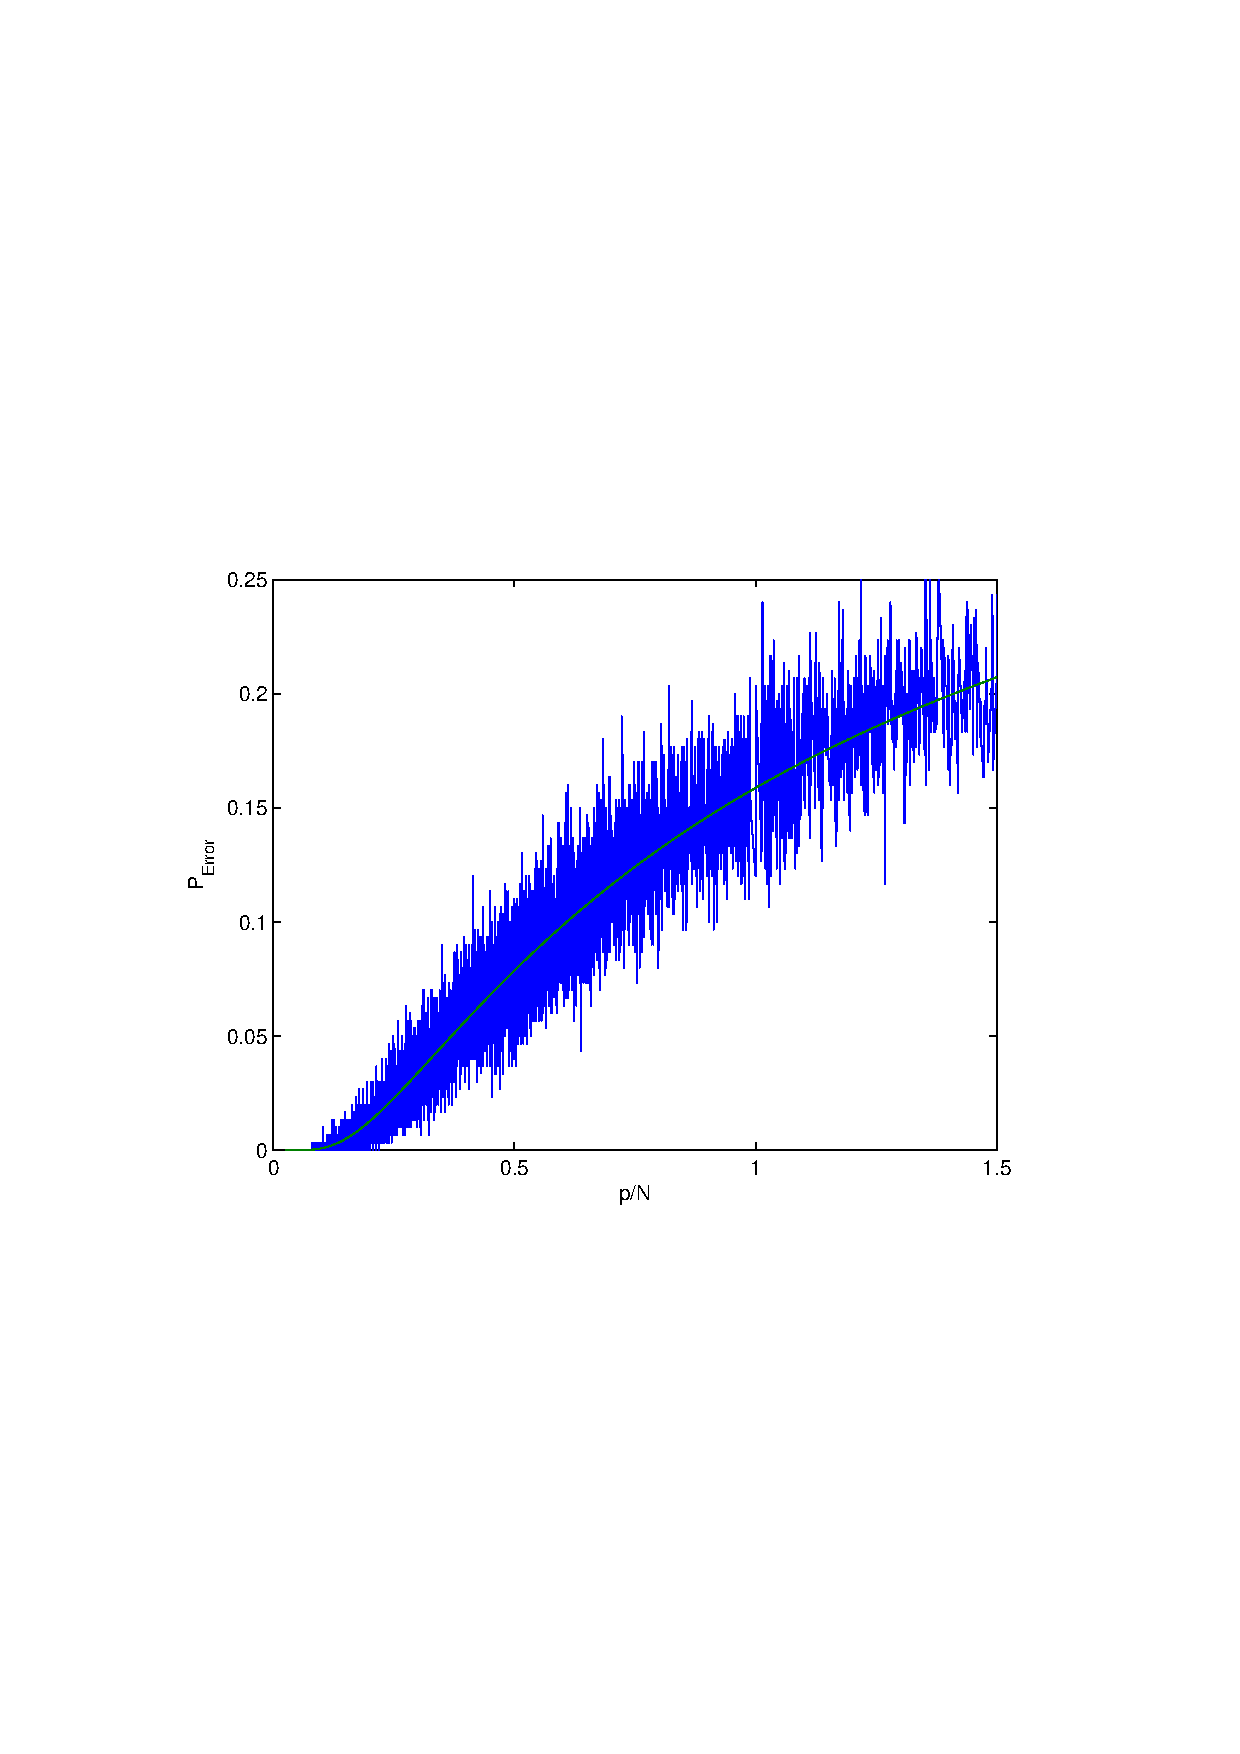
\includegraphics[width=12cm]{uppg1.pdf}
\caption{\label{uppg1} A plot of the result of problem 1, based on 7571
points of data, where weights $w_{ii} = 0$. The value $P_{Error}$ is the
probability that a neuron is incorrectly flipped on the first iteration of
the Neural Network.  The value $p$ is the number of \emph{random patterns}
stored in the network and $N$ is the number of neurons. The green line is
the theoretical values.}
\end{figure}

\begin{figure}\centering
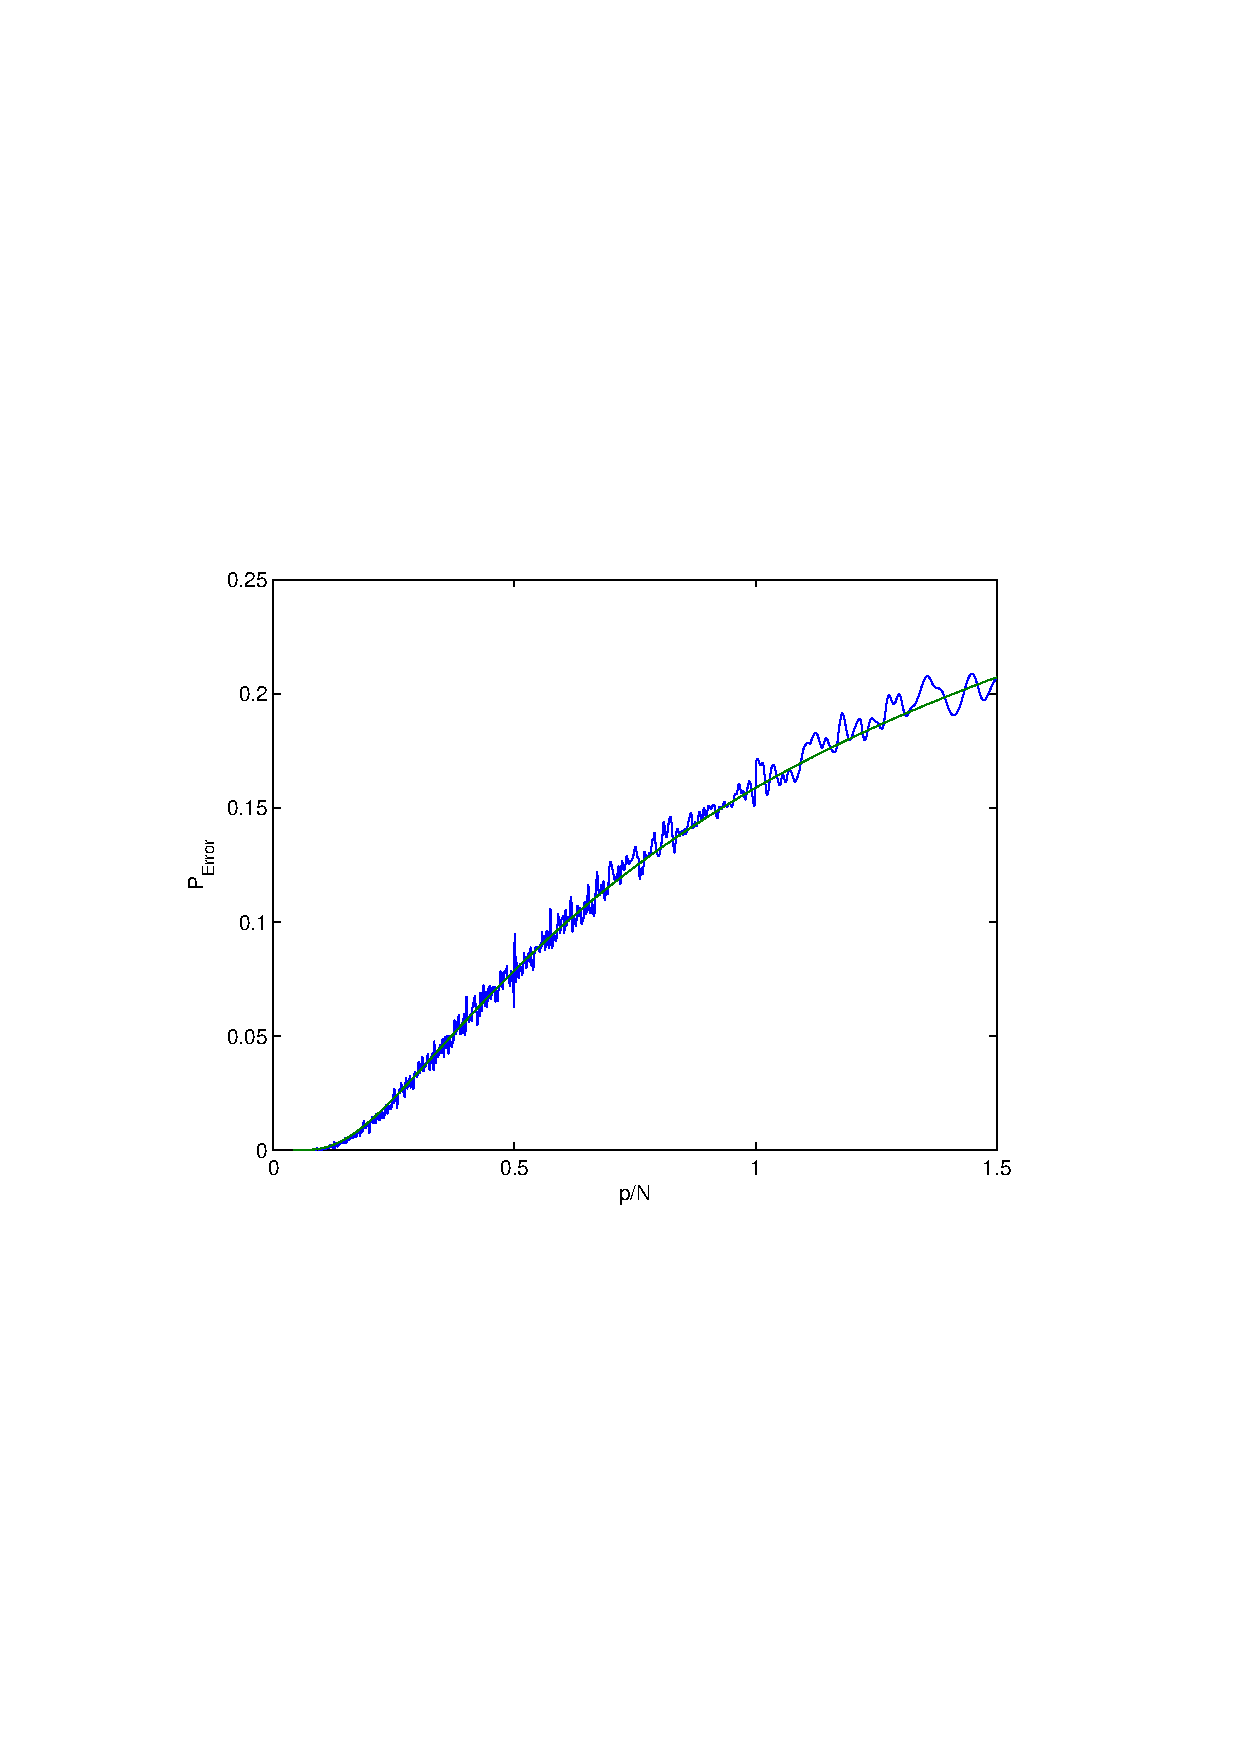
\includegraphics[width=12cm]{uppg1_smooth.pdf}
\caption{\label{uppg1_smooth} The same data as Figure \ref{uppg1} smoothed out using the method described in section \ref{inMatlab1}, so in the end it is based on 200 fewer data points.}
\end{figure}


\subsubsection{Limitations}

The simulation was done in a limited range for both $p$, $N$ and $p/N$, so if there is any significantly different trends outside these intervals, we cannot see them.

Furthermore, since the random samples was generated uniformly distributed over $p$ and $N$, the resolution is not the same everywhere in the plots. In particular, the borders are especially low-res. On the other hand, we have used ridiculously many samples, so this should not matter.

As a smooth representation of the data points, a spline might have been better. I have not yet tested this.

\subsection{Code}
 
\begin{verbatim}
$ g++ -o uppg1 uppg1.cpp nn_common.cpp
$ ./uppg1 >> uppg1_new
$ matlab -r uppg1
\end{verbatim}

\section{Deterministic Hopfield model continued}

\subsection{Problem}
This is the same problem as in section \ref{dhm} except that now the Hebb
rule is used for all $w_{ij}$ including $i = j$.

\subsection{Approach}
The approach for this problem is identical to the one used for problem 1,
except that the code that sets weights $w_{ii}$ to zero is
removed.\footnote{Furthermore a few more trials where done per point, but
not significantly different.} 

In this case, the theoretical value of $P_{Error}$ is
\begin{equation} \label{theoretical2}
P_{Error} = \frac{1}{2} \operatorname{erfc}(\frac{1 + \frac{p}{N}}{\sqrt{2 \frac{p}{N}}}).
\end{equation}
The deduction of \eqref{theoretical2} is based on the
calculation for $w_{ii} = 0$ and can be seen in detail in Appendix B.

\subsection{Result and discussion}
The results of this simulation is seen figures \ref{uppg2} and
\ref{uppg2_smooth}. As above Figure \ref{uppg2_smooth} is a smoothed out
version of \ref{uppg2}, and the blue curves shows the result of the
simulations and the green curve shows the theoretical values.

Once again the theory matches the experiments very good. However, this time
the theoretical values seems to slightly overestimate the experimental
result. This may be due to the assumption that $p$ is sufficiently large, so
$\frac{p-1}{N} \approx \frac{p}{N}$. The more exact formula for small $p$ would (as expected) generate smaller values.

As we can see the figures we have a much lower value of $P_{Error}$ in this
case then when $w_{ii} =0$. This does not say anything about the long-term
result though. Another interesting property is that after a certain point
the error probability actually decreases. This does not say anything about
long term probability either.

\begin{figure}\centering
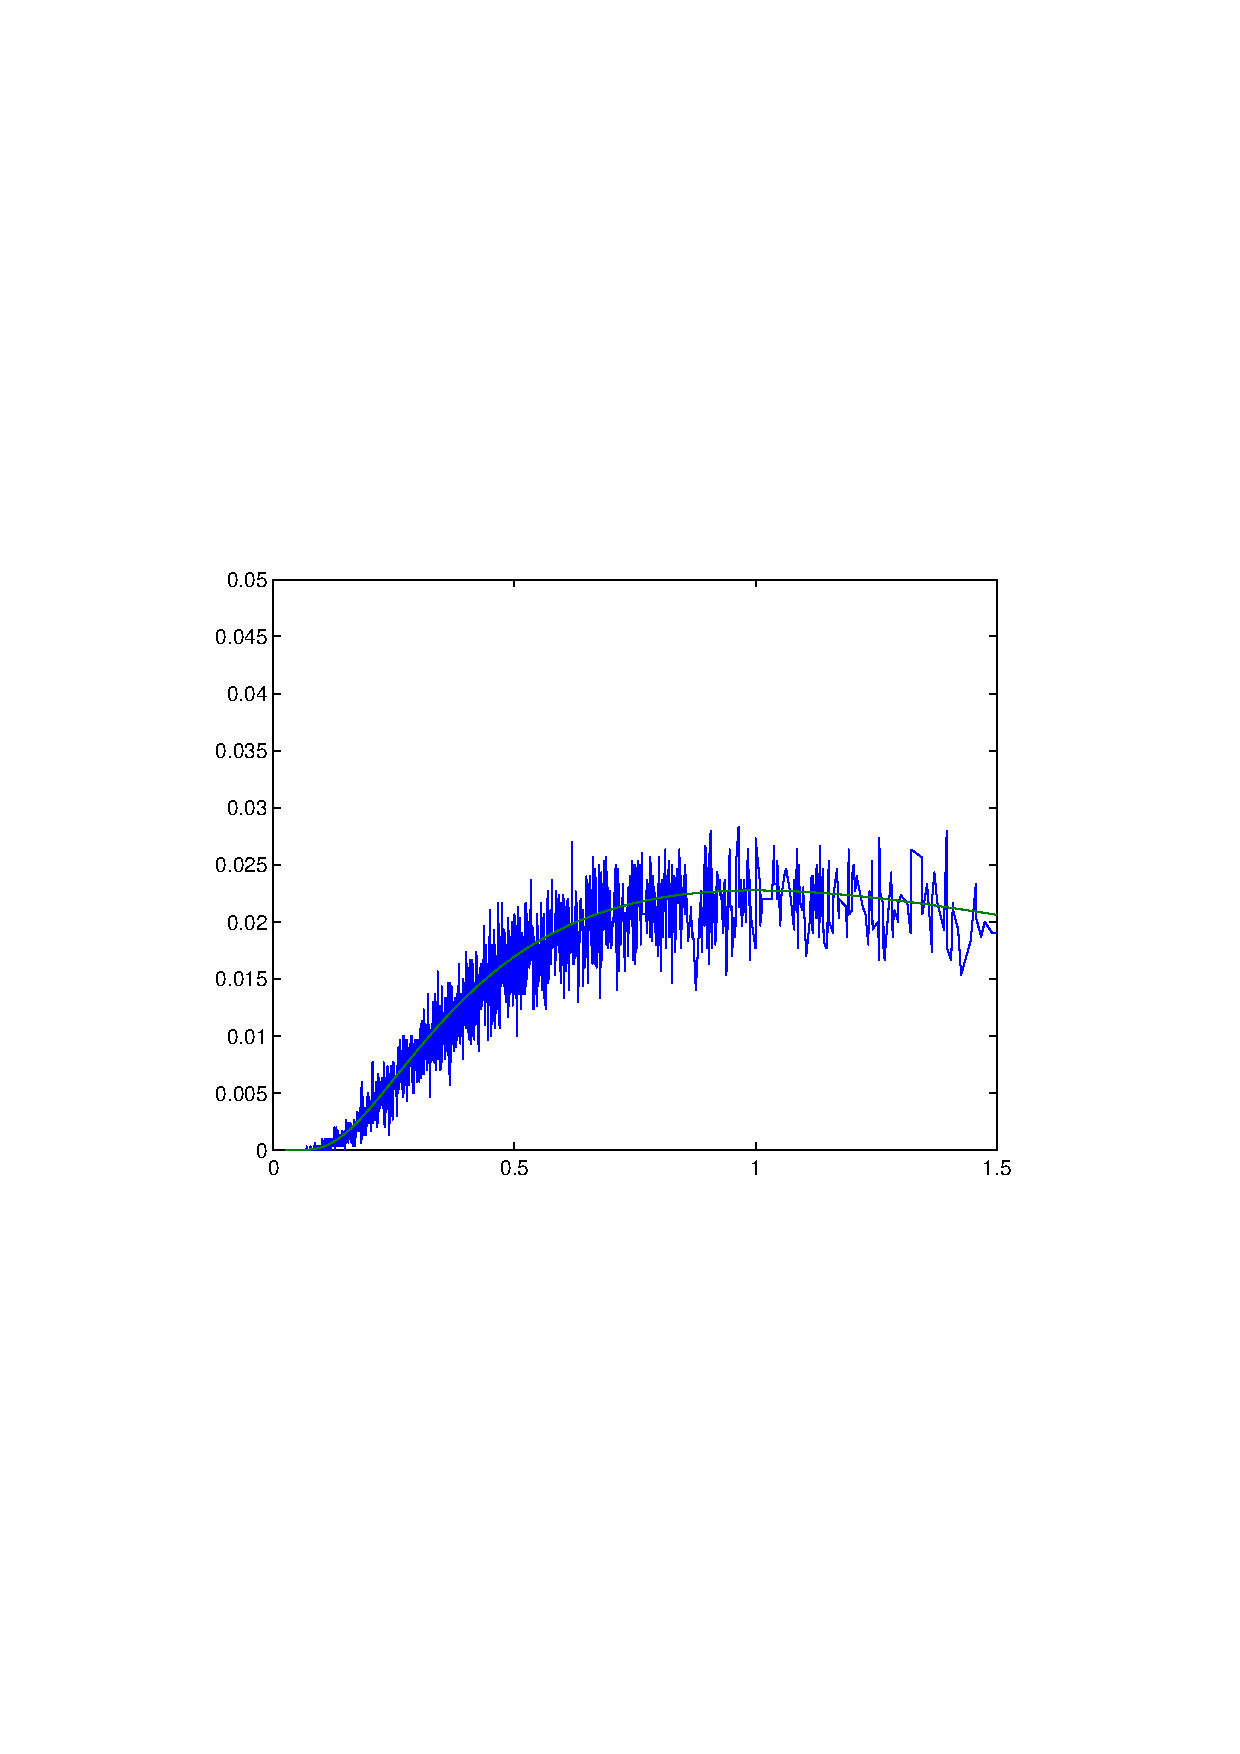
\includegraphics[width=12cm]{uppg2.pdf}
\caption{\label{uppg2} A plot of the result of problem 2, where weights
$w_{ii} \neq 0$. The value $P_{Error}$ is the probability that a neuron is
incorrectly flipped on the first iteration of the Neural Network.  The value
$p$ is the number of \emph{random patterns} stored in the network and $N$ is
the number of neurons. The green line is the theoretical values.}
\end{figure}

\begin{figure}\centering
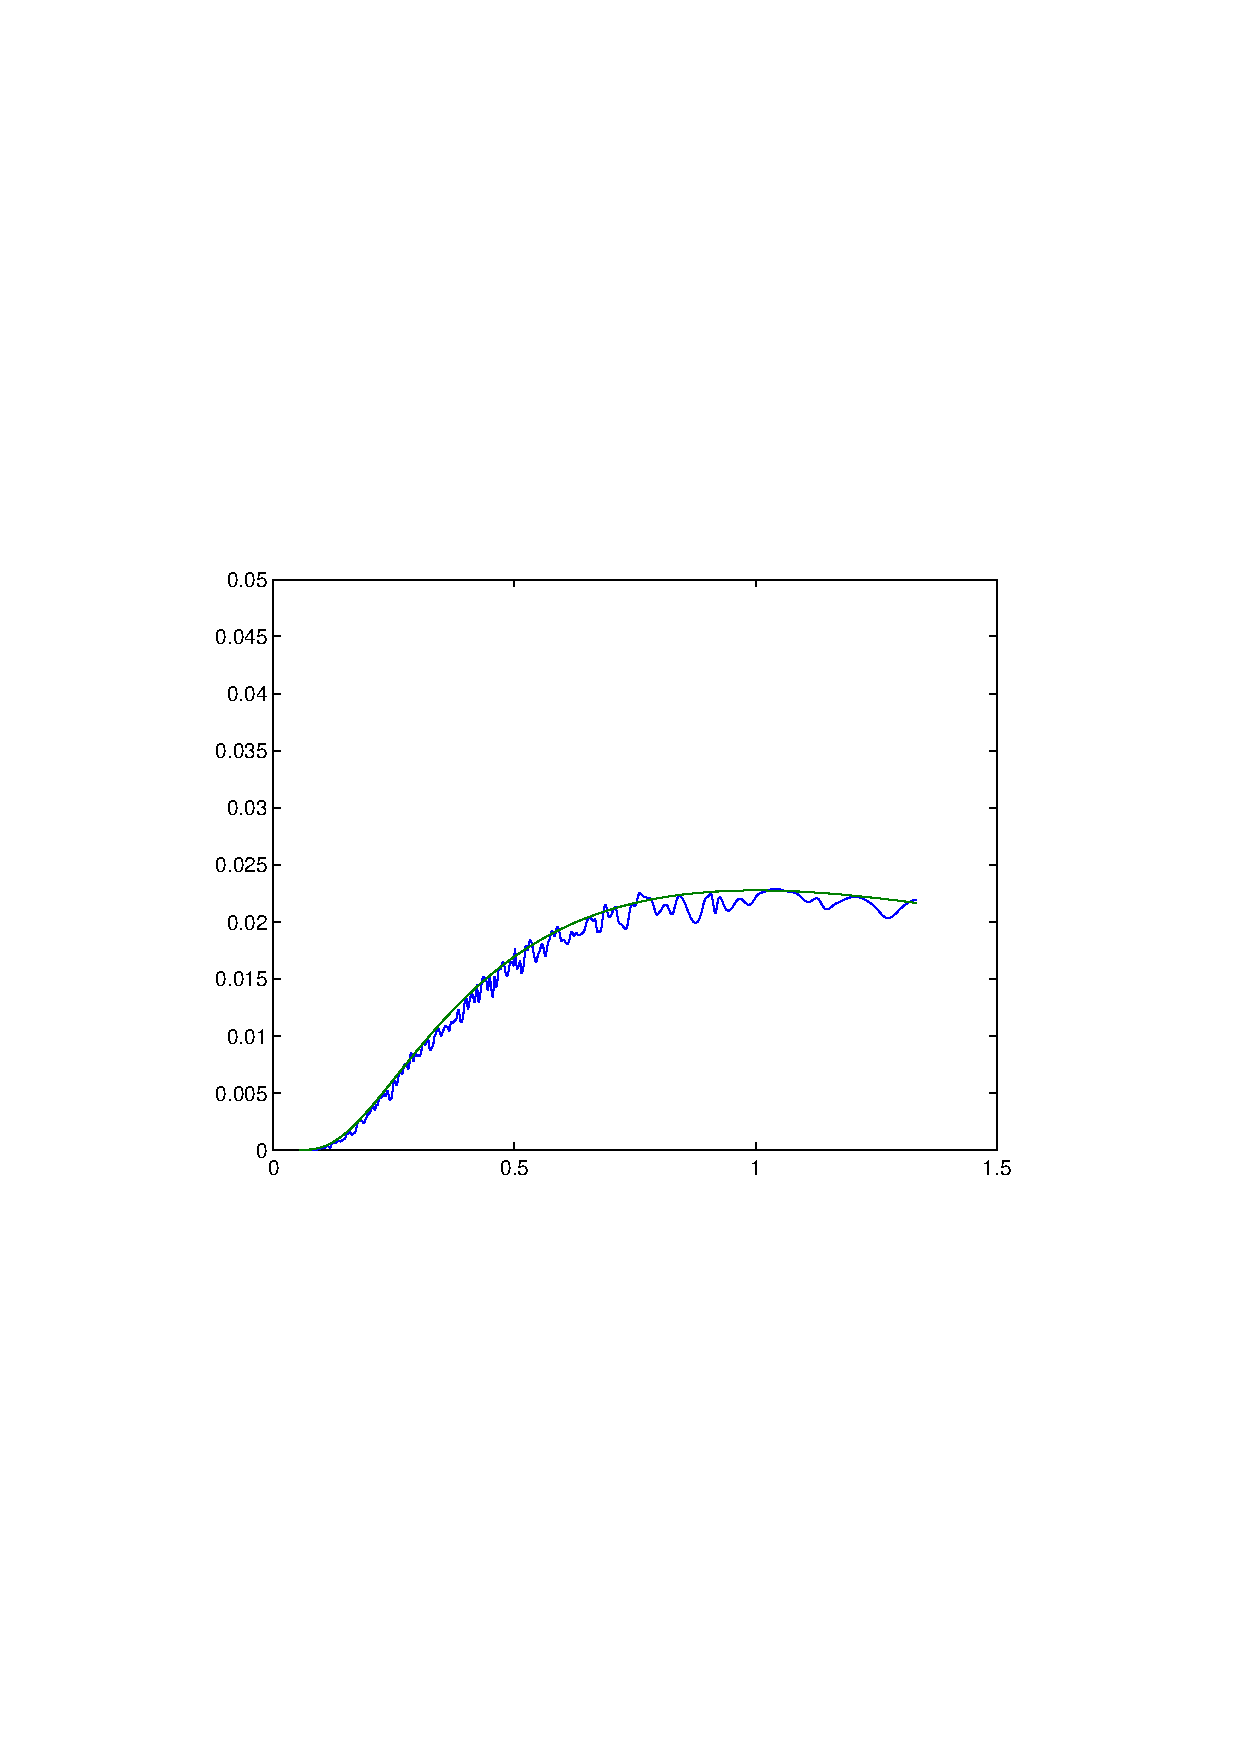
\includegraphics[width=12cm]{uppg2_smooth.pdf}
\caption{\label{uppg2_smooth} The same data as Figure \ref{uppg2} smoothed out using the method described in section \ref{inMatlab1} .}
\end{figure}

\subsection{Code}

\begin{verbatim}
$ g++ -o uppg2 -DUPPG2 uppg1.cpp nn_common.cpp
$ ./uppg2 >> uppg2_new
$ matlab -r uppg2
\end{verbatim}

\section{Stochastic Hopfield model}
\subsection{Problem}
Write a program that implements the Hopfield model with stochastic updating.
Use the following values: number of neurons $N = 200$, noise level
$\beta^{-1} = 0.5$ and number of (random) patterns $p$ is either $=5$ or
$=40$. Plot order parameter $m_1$ as function of time $t$. Describe results for $p = 5$ and compare results with $p=40$

\subsection{Approach}
The value $m_1(t)$ is defined as $m_1(t) = \frac{1}{N} \sum_{i =1}^N
\zeta^{(1)}_i  S_i(t)$, where $N$ is the total number of neurons,
$\zeta^{(\mu)}_i$ is pattern $\mu$ at position $i$ and $S_i(t)$ is the state
of neuron $i$ at time $t$.

The same general approach that is described in section \ref{app1} is used. The stochastic update rule is implemented by replacing the function $\operatorname{sgn}(b)$ with a function which returns $1$ or $-1$ with probability
$$ g(b) = \frac{1}{1 + \operatorname{e}^{-2 \beta b}}. $$

\subsubsection{In C++}
The code starts by initialize the patterns randomly.
Then on each timestep the value of $m_1$ is printed out to standard output
followed by a tab. This is done for 10000 timesteps, and then a newline is
appended. This whole process is then repeated 100 times.

\subsubsection{In MATLAB}
First the result for both $p=5$ and $p=40$ is imported, then the mean over
all simulations is taken per timestep and value of $p$. Then both results are plotted.

\subsection{Result and discussion}
In the green curve in Figure \ref{uppg3} and in Figure \ref{uppg3_5}
we can see that the process is very stable for $p=5$, you can see that
$\lim_{t \to \infty} m_1(t) \approx 1$. This is \emph{not} the case for $p
= 40$ (Blue curve in Figure \ref{uppg3} and Figure \ref{uppg3_40}). In this case we it seems more like $\lim_{t \to \infty} m_1(t) \approx 0$.

\begin{figure}\centering
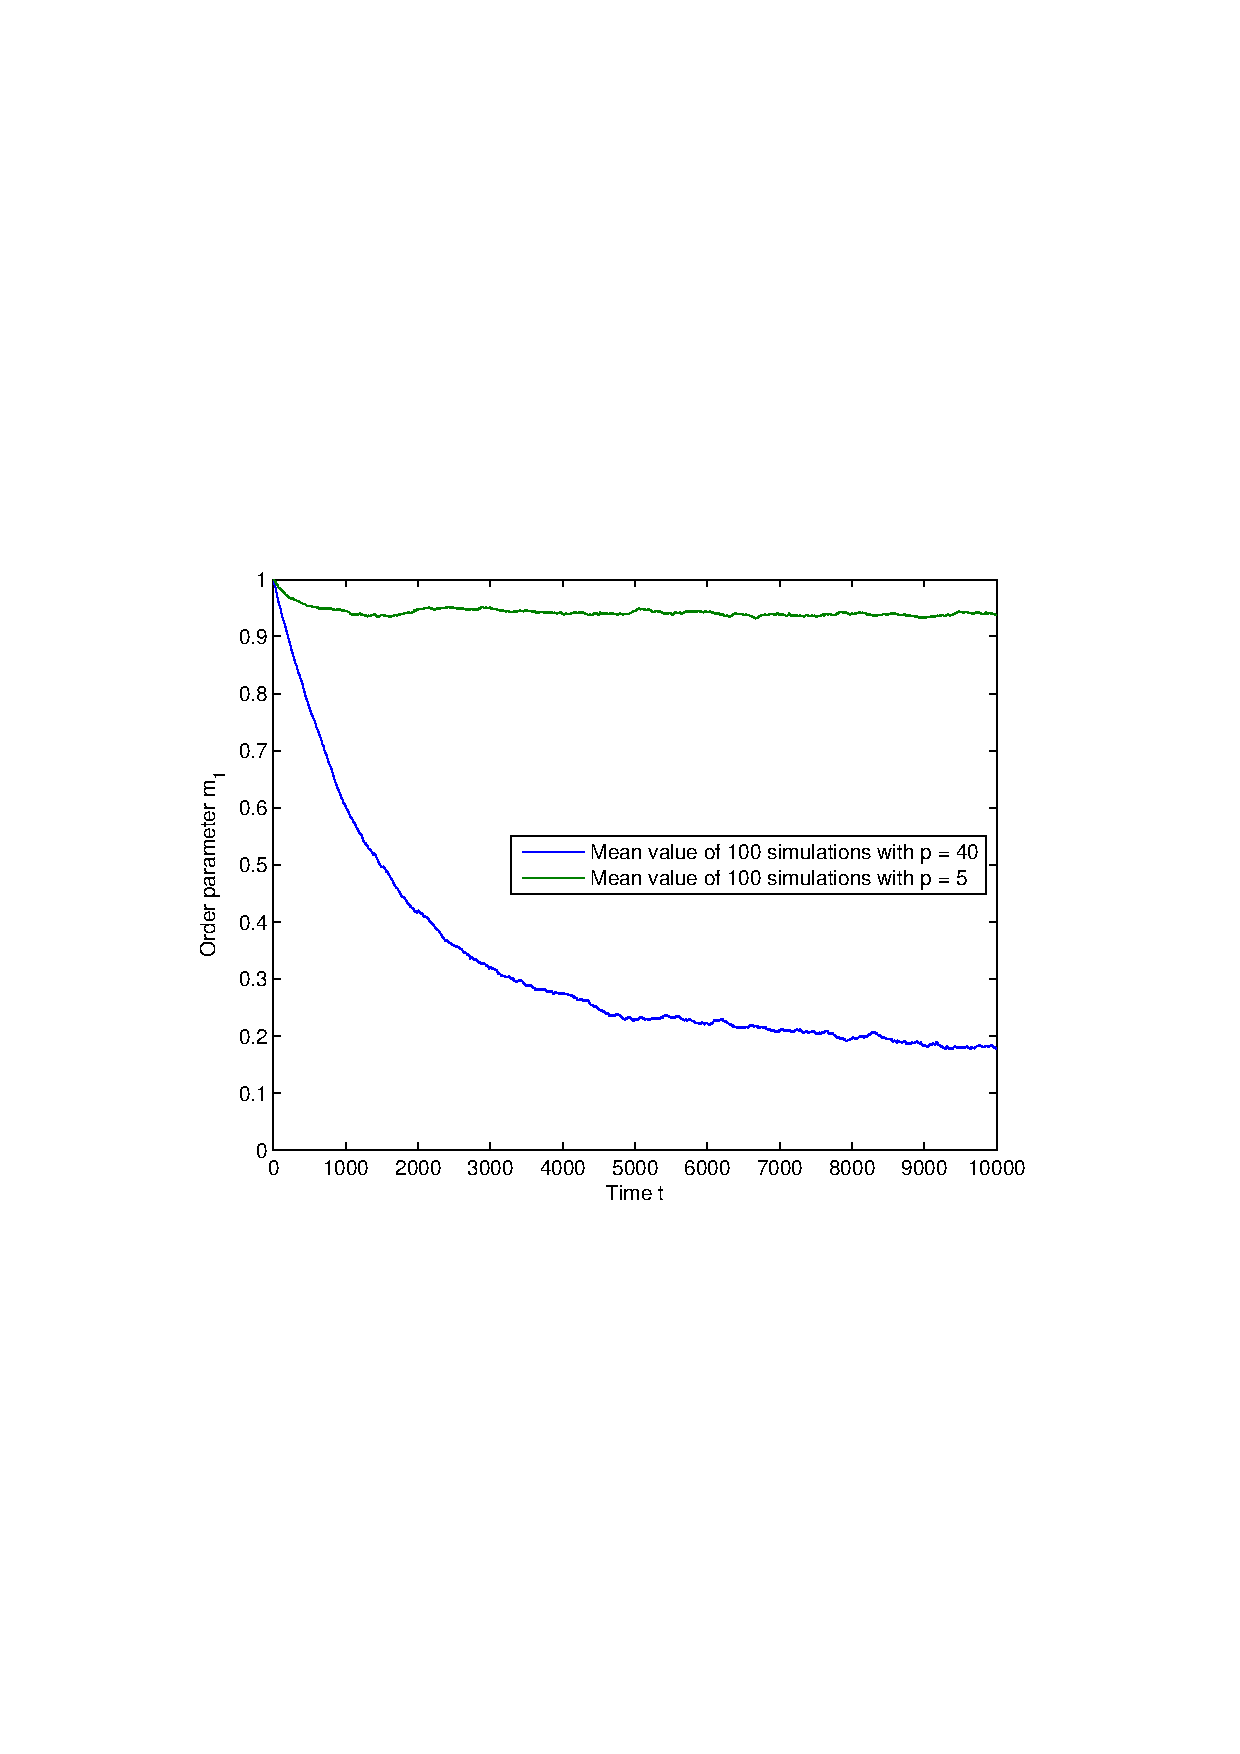
\includegraphics[width=\textwidth]{uppg3.pdf}
\caption{\label{uppg3} Plot of the mean value over 100 simulations of the
order parameter for the first pattern, $m_1$, as a function of time, using
a stochastic Hopfield model, with the number of neuron $N = 200$, the
noise level $\beta^{-1} = 0.5$ and the number of patterns $p = 40$ and $p=5$
respectively. All the patterns are randomized and the network is initially fed with pattern 1. }
\end{figure}

\begin{figure}\centering
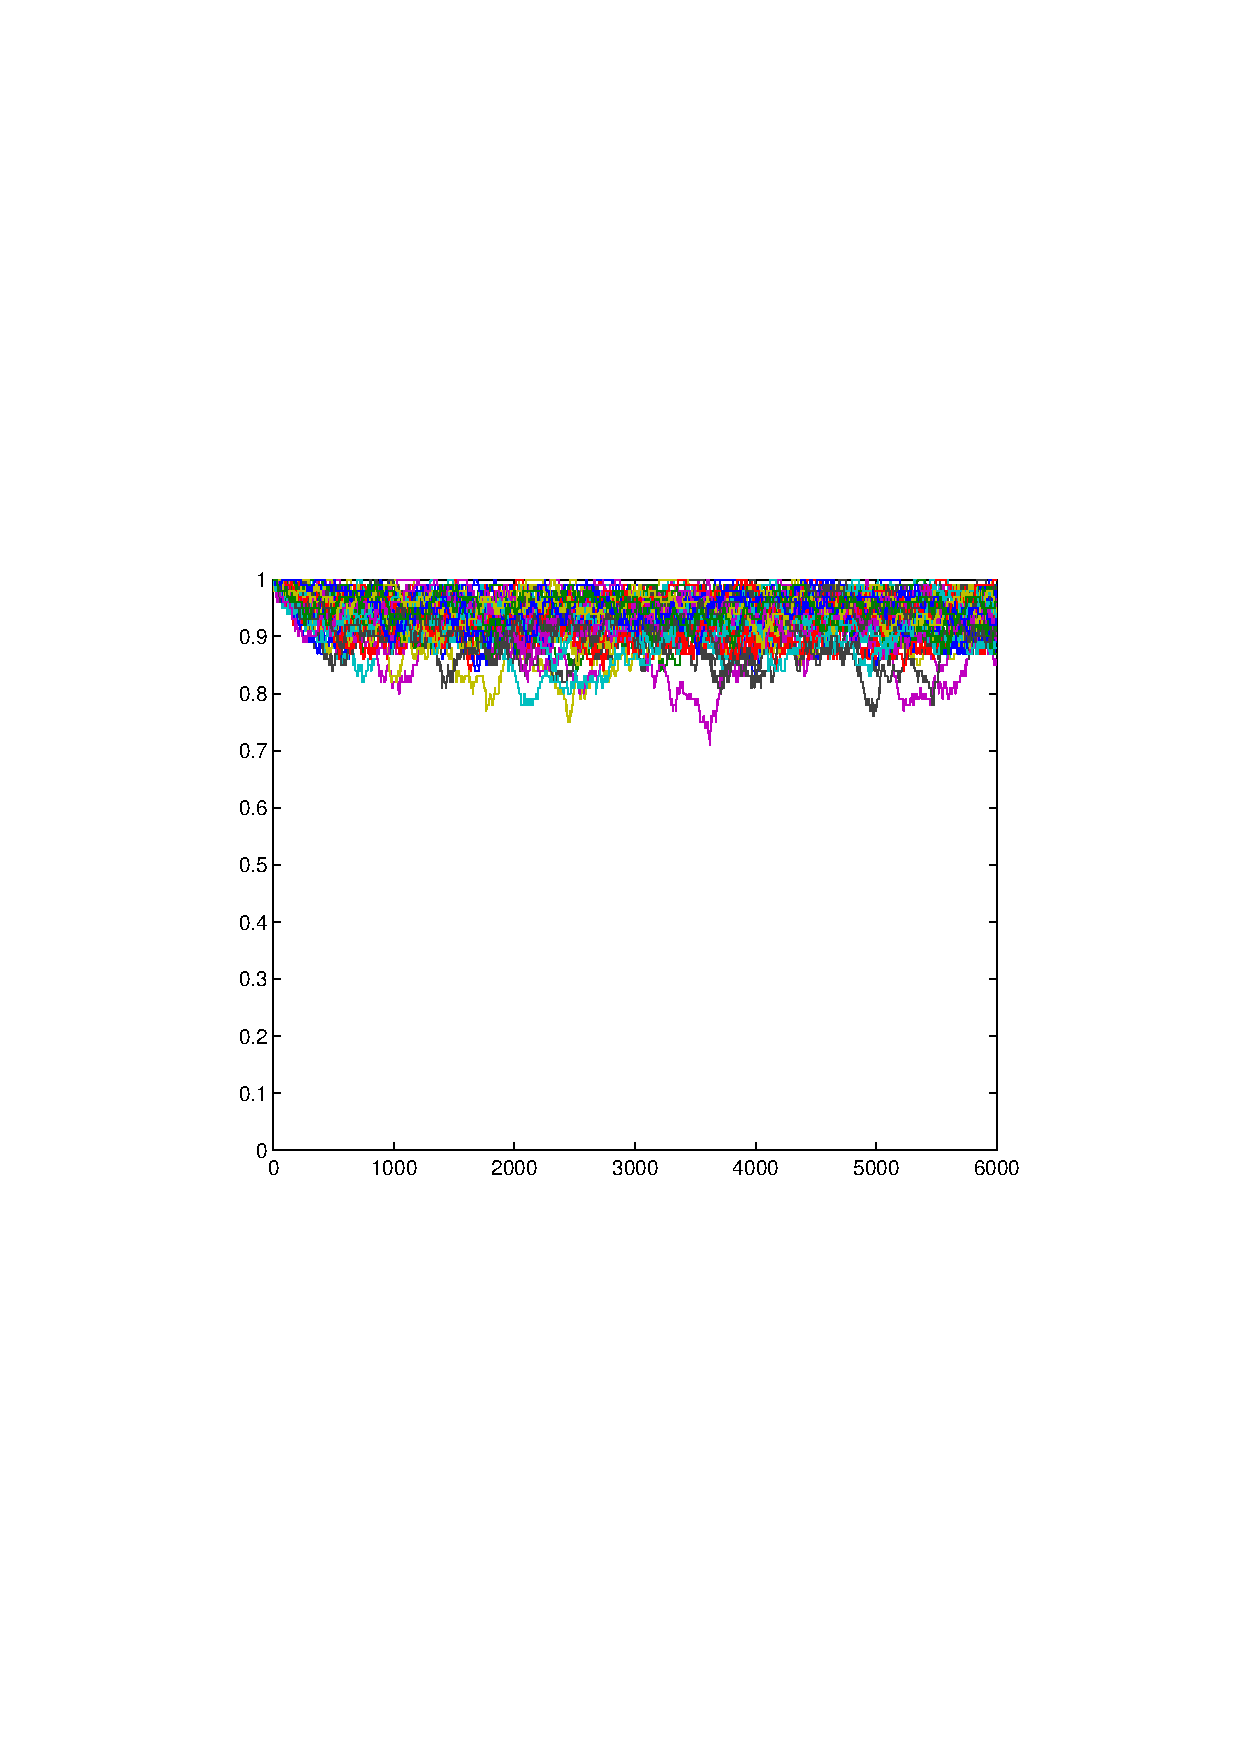
\includegraphics[width=\textwidth]{uppg3_5.pdf}
\caption{\label{uppg3_5} Plot of 100 simulations of the
order parameter for the first pattern, $m_1$, as a function of time, using
a stochastic Hopfield model, with the number of neuron $N = 200$, the
noise level $\beta^{-1} = 0.5$ and the number of patterns $p=5$ . All the
patterns are randomized and the network is initially fed with pattern 1. }
\end{figure}
\begin{figure}\centering
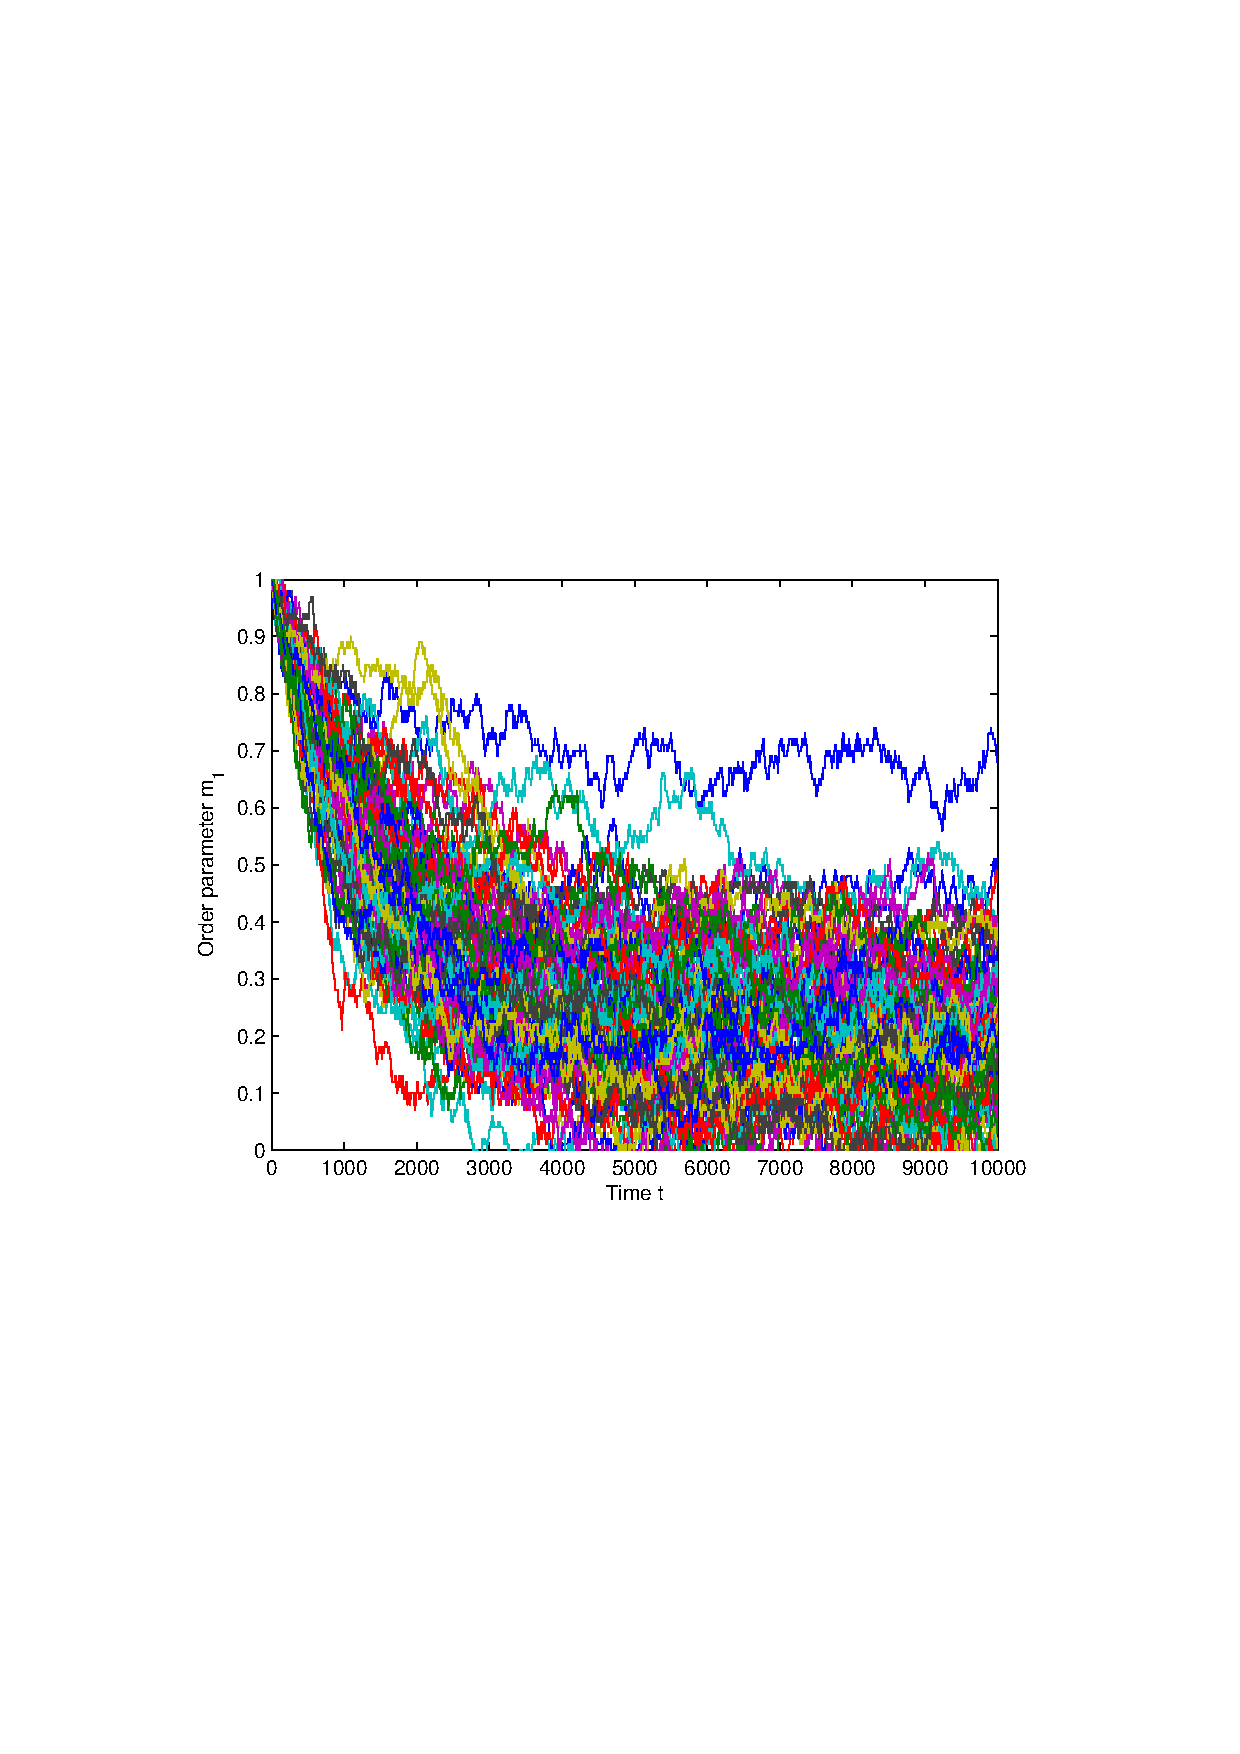
\includegraphics[width=\textwidth]{uppg3_40.pdf}
\caption{\label{uppg3_40} Plot of 100 simulations of the
order parameter for the first pattern, $m_1$, as a function of time, using
a stochastic Hopfield model, with the number of neuron $N = 200$, the
noise level $\beta^{-1} = 0.5$ and the number of patterns $p=40$ . All the
patterns are randomized and the network is initially fed with pattern 1. }
\end{figure}
\subsection{Code}

\begin{verbatim}
$ g++ -Dforty  uppg3.cpp nn_common.cpp -o uppg3_40 
$ g++ -Dfive  uppg3.cpp nn_common.cpp -o uppg3_5
$ ./uppg3_40 > uppg3_40.data
$ ./uppg3_5 > uppg3_5.data
$ matlab -r uppg3
\end{verbatim}

\newpage

\appendix

\section{Source code}

\subsection{C++}

\subsubsection{uppg1.cpp}
\lstinputlisting{../uppg1.cpp}

\subsubsection{uppg1.hpp}
\lstinputlisting{../uppg1.hpp}

\subsubsection{uppg3.cpp}
\lstinputlisting{../uppg3.cpp}

\subsubsection{uppg3.hpp}
\lstinputlisting{../uppg3.hpp}

\subsubsection{nn\_common.cpp}
\lstinputlisting{../nn_common.cpp}

\subsubsection{nn\_common.hpp}
\lstinputlisting{../nn_common.hpp}

\subsection{MATLAB}

\subsubsection{uppg1.m}
\lstinputlisting{../uppg1.m}

\subsubsection{uppg2.m}
\lstinputlisting{../uppg2.m}


\subsubsection{uppg3.m}
\lstinputlisting{../uppg3.m}


\end{document}
